\IEEEPARstart{A}{} diferencia de trabajos previos, la experimentaci\'on de este
trabajo es mucho m\'as explorativa que basada en hip\'otesis a confirmar.
Claramente, al comenzar la experimentaci\'on se tuvieron algunas hip\'otesis
(detalladas a continuaci\'on), pero se comenz\'o esta tarea m\'as con un
objetivo de observar que ocurre con los m\'etodos propuestos seg\'un algunas
variables que fueron identificadas.

\par A su vez, el dominio de este trabajo es m\'as subjetivo, si se quiere, que
los trabajos previos. Es decir, al interpolar cuadros (o \emph{frames}) de un
video, nos interesa como es la percepci\'on de la audiencia del mismo. ¿Se nota
la interpolaci\'on?¿Da una sensaci\'on anormal?¿No se nota, quiz\'as?.
B\'asicamente: el resultado obtenido, ¿es bueno?. Claramente esto es muy
subjetivo y dependiente, entre otras cosas, de la persona que emite el juicio.
As\'i pues, se tuvo que buscar alguna forma de comparar los distintos m\'etodos
de la forma m\'as objetiva posible. Pero tampoco se quizo dejar de lado este
an\'alisis ''subjetivo'', que al fin y al cabo, es el m\'as importante.

\par A lo largo de esta secci\'on comenzaremos primero enunciando las
hip\'otesis que se pudieron enunciar antes de comenzar, la explicaci\'on de las
variables con las que se experiment\'o (derivadas a partir de las hip\'otesis),
para luego pasar a la experimentaci\'on misma (con un m\'inimo an\'alisis de
correctitud), d\'onde se analizan los aspectos cu\'antitativos y cualitativos
(y como se a explicado, algunos de estos \'ultimos de manera subjetiva).
Finalmente, realizamos una an\'alisis breve de los \emph{artifacts} frutos de
los videos interpolados y terminamos esta secci\'on indicando ciertos trabajos
a futuros que podr\'ian ser de inter\'es.

%---------------------------------------------------------------
\subsection{Hip\'otesis}
\IEEEPARstart{E}{N} esta parte del trabajo se explican algunas de las hip\'otesis
que pudieron ser formuladas al pensar en el problema. Como ya se ha dicho, la
naturaleza de este trabajo ha sido m\'as exploratoria, pero a\'un as\'i se
comenz\'o el mismo con algunas conjeturas y nociones de lo que deb\'ia ocurrir.

\begin{enumerate}
    \item\begin{LaTeXdescription}
        \item[Hip\'otesis] saraza

        \item[Motivaci\'on] saraza
    \end{LaTeXdescription}
\end{enumerate}


%---------------------------------------------------------------
\subsection{Variables Identificadas para la Experimentaci\'on}
\IEEEPARstart{A}{} partir de las hip\'otesis enunciadas, se determinaron
ciertas caracter\'isticas y par\'ametros que posiblemente afecten a la calidad
de las interpolaciones aplicadas a los videos. Estas son:

\begin{LaTeXdescription}
    \item[Frames Interpolados] La cantidad de frames artificalmente generados
        que ser\'an insertados entre cada par de frames del video original. Se
        consideron 4 alternativas para esta variable: 1, 2, 5 o 10 frames.
        Agregar de a 1 frame cada virtualmente duplica la cantidad de frames
        del video original, con lo cual si se mantiene el \emph{ratio de
        reproducci\'on}\footnote{Frames per second.} se estar\'ia obteniendo el
        efecto de reproducir a la ''mitad'' de la velocidad original. Se
        consider\'o algunas alternativas m\'as, aunque es d\'ificil imaginar
        alg\'un contexto donde se busque reproducir artificalmente el efecto de
        \emph{c\'amara lenta} con algo m\'as de 5 frames.\medskip

    \item[M\'etodo de Interpolaci\'on] Tenemos 3 formas/m\'etodos de generar
        los frames interpolados: Vecino m\'as Cercano, Interpolaci\'on Lineal,
        Interpolaci\'on C\'ubica o Spline. Claramente cada uno de ellos funciona
        de forma distinta, como ya se ha explicado. As\'i pues, la elecci\'on
        del m\'etodo deber\'ia afectar a los frames generados artificialmente,
        ya que dificilmente en un caso de uso real los m\'etodos devuelvan un
        frame artificial id\'entico.\medskip

    \item[Tama\~no de Bloque (splines)] El m\'etodo de spline puede pensarse
        como aplicado a todo el video, o se podr\'ian aplicar a distintos
        bloques a lo largo del video (generando disintos splines por cada
        bloque del video).  Parte de los objetivos de la experimentaci\'on es
        ver si esto afecta a los resultados de alguna manera. Los valores
        considerados fueron 4, 8, 16 y 32 frames (m\'as el caso de aplicar el
        m\'etodo a todo el video).\medskip

    \item[Resoluci\'on del Video] ¿La resoluci\'on del video afecta a los
        m\'etodos de alguna manera?¿Es acaso alguno de ellos (o todos) m\'as
        preciso para resoluciones mayores?\footnote{Se experiment\'o con los
        mismos videos en 2 resoluciones diferentes, pero por cuestiones de
        tiempo los resultados de las resoluciones m\'as grandes no pudieron ser
        analizadas.}.\medskip

    \item[Tipo Movimiento grabado por la C\'amara] A partir de una c\'amara uno
        podr\'ia grabar algo est\'atico o con poco movimiento, como por ejemplo
        el crecimiento de la vida vegetal\footnote{O a la defensa de Platense
        jugando al \emph{offside}}, o algo con m\'as movimiento como por
        ejemplo una carrera de autos o un evento deportivo\footnote{No, no
        quedamos manija luego del TP2}.  As\'i pues, dados los tiempos de este
        trabajo, decidimos hacer una bipartici\'on de los posibles videos
        respecto de esta caracter\'istica: videos que graban cosas est\'aticas
        como videos que filman situaciones donde hay movimiento.  Hay
        distinciones que ser\'ian interesantes tener en cuenta, como por
        ejemplo si los movimientos son abruptos o suaves, pero nuevamente los
        tiempos para confeccionar esta trabajo no permitieron dicho
        an\'alisis.\medskip

    \item[Tipo de Movimiento de la C\'amara] Al igual que en el item anterior,
        bien se puede considerar los movimientos de la c\'amara que efect\'ua
        la filmaci\'on. De hecho, podr\'ia llegar a considerarse que si se
        analiza el movimiento de un video, no importa si el mismo proviene de
        mover la c\'amara o de filmar algo que efectivamente cambie de
        posici\'on. A\'un as\'i, dado que en este aspecto en realidad estamos
        explorando como se comportan los m\'etodos propuestos, se decidi\'o
        realizar una partici\'on similar al caso previo para los movimientos
        de la c\'amara: videos donde la c\'amara est\'e fija y videos donde
        la misma presente alg\'un tipo de movimiento. Nuevamente entra en juego
        otras distinciones respecto de como son estos movimientos que no
        pudieron ser evaluadas por las limintantes de tiempo ya
        mencionadas.\medskip
\end{LaTeXdescription}

\par Estas son algunas de las variables que se podr\'ian en tener en cuenta (en
particular las que se tuvieron en cuenta en este trabajo), pero no son las
\'unicas. Por dar un ejemplo, una variable con la que no se trabaj\'o fue con
los videos que cambi\'an de c\'amara, donde se pas\'a de un tipo de im\'agen a
otra de form\'a rotunda en frames contiguos (podr\'ia haber alg\'un tipo de
transici\'on tambi\'en, que ser\'ia otro caso a estudiar). Fue meramente por
cuestiones de tiempo que se decidi\'o limitar el enfoque de este trabajo a las
variables/par\'ametros enunciados.


%---------------------------------------------------------------
\subsection{Metodolog\'ia de Experimentaci\'on}\label{subsec:metodologia}
Durante la experimentaci\'on, y dada la naturaleza de la misma,
se sigui\'o una misma metodolog\'ia para recabar la informaci\'on necesaria para
ser luego analizada.

\par En primer lugar se decidi\'o trabajar con im\'agenes en escala de grises o,
coloquialmente llamado \emph{blanco y negro}. Esto es as\'i ya que dentro del
alcance de nuestro trabajo, estamos estudiando (principalmente) la correctitud
de los frames interpolados. Si se tuvieran en cuenta los colores, se tendr\'ia
la complicaci\'on del error agregado de interpolar los canales de colores por
separado, lo cual escapa a los objetivos del trabajo (adem\'as de tener la
limitante del tiempo para realizar este trabajo.). Resumiendo, se tom\'o esta
decisi\'on para simplificar y enfocar m\'as el an\'alisis a realizar.

\par La forma en la que se presentar\'an los resultados m\'as adelante nada
tiene que ver con el orden en el que se realiz\'o la experimentaci\'on.

\par De la secci\'on anterior se puede observar que existen dos variables que
nos indican (o limitan) los tipos de videos con los que trabajaremos. Estas dos
variables no son otra que las diferentes combinaci\'on del tipo de movimiento
filmado y de la c\'amara que realiza la grabaci\'on. As\'i pues, se termin\'o
teniendo cuatro combinaci\'ones posibles: \emph{c\'amara fija-im\'agen fija},
\emph{c\'amara fija-im\'agen m\'ovil}, \emph{c\'amara m\'ovil-im\'agen fija} y
\emph{c\'amara m\'ovio-im\'agen m\'ovil}\footnote{Existen matices en estas
combinaciones. Por ejemplo, \emph{la suavidad} de los movimientos, que podr\'ian
variar en intensidad yendo de suaves a bruscos. Nuevamente, por cuestiones de
tiempo se decidi\'o no incursionar en estos aspectos.}.

\par Para cada una de estas categor\'ias de videos, se efectu\'o la
interpolaci\'on con los 3 m\'etodos expuestos y todas sus posibles combinaciones
de par\'ametros (cantidad de frames a interpolar entre frame y frame, y en el
caso de spline el tama\~no de bloque.). Para luego poder hacer un an\'alisis
objetivo de la calidad de los frames interpolados resultantes, lo que se hizo
fue remover de los videos originales una cantidad calculada\footnote{En base
a la cantidad de frames a interpolar.} de frames antes de interpolar el mismo.
De esta manera se puede comparar los frames interpolados resultantes con los
frames originales (los que fueron removidos previos al procesamiento), que no
son otra cosa que el resultado que uno quisiera obtener de la interpolaci\'on.

\par Luego se realizan los an\'alisis de los m\'etodos independientemente de los
dem\'as m\'etodos, es decir que analizamos los resultados obtenidos de cada
m\'etodo respecto de sus par\'ametros de entrada.

\par Continuamos realizando un an\'alisis de m\'etodo versus m\'etodo, para
los mismos par\'ametros (en el caso de splines, al tener 2 par\'ametros de
entrada\footnote{Cantidad de bloques a interpolar y tama\~no de bloque.} se
tuvieron que utilizar resultados obtenidos del an\'alisis del m\'etodo
realizado previamente).

\par Por \'ultimo, antes de terminar enunciando las conclusiones obtenidas para
el tipo de video estudiado, se generaron unos videos que realizan la
comparativa frame a frame de la diferencia entre el frame del video original y
su contraparte interpolada para luego ser estudiados (visualizado en forma de
\emph{heatmap}). La idea de esto es la de encontrar en que zonas de los frames,
respecto de lo que ocurre en el video, genera problemas para los m\'etodos
estudiados.

\par Las m\'etricas utilizadas para los an\'alisis de los m\'etodos no son otras
que las sugeridas por la c\'atedra: el \emph{Error Cuadr\'atico
Medio}~\cite{mse} y el \emph{Peak Signal to Noise Ratio}~\cite{psnr}. El primero
es una medida de error entre un valor (en nuestro caso, un frame) estimado y lo
que es estimado (el frame original). Mientras que el \emph{PSNR} es un ratio
que toma en cuenta el \emph{ECM} y el valor m\'aximo siendo
estimado\footnote{Oriundo del an\'alisis de se\~nales, donde indica la
relaci\'on entre la potencia m\'axima de una se\~nal y la potencia del ruido
que la afecta.}. Justamente el PSNR es utilizado para cuantificar la calidad de
la reconstrucci\'on de una se\~nal (o en nuestro caso, de un frame), un alto
valor del mismo del mismo indica mayor calidad de la reconstrucci\'on (aunque
se debe tener cierto cuidado en los casos donde existe compresi\'on de datos
involucrada, caso que no aplica a este trabajo). Tambi\'en se usaron los
valores medios, desv\'io est\'andard, m\'aximo y m\'inimo del ECM para realizar
comparaciones para el mismo m\'etodo y sus diferentes par\'ametros, como as\'i
tambi\'en entre los distintos m\'etodos.

\par Vale la pena aclarar que en las conclusiones generales es donde tambi\'en
se realiza un an\'alisis m\'as subjetivo, basado en la percepci\'on de los
autores de este trabajo. Claramente esta no es una muestra lo suficientemente
alta de las posibles audiencias de los videos, pero alcanza dado el objetivo
did\'actico del trabajo.

\par Para concluir con esta secci\'on, agregamos a su vez que se realizaron
otros experimentos m\'as puntuales para analizar los aspectos de correctitud de
los m\'etodos (m\'inimamente) y del tiempo de c\'omputo, como as\'i tambi\'en
una comparativa de como los m\'etodos se ven afectados seg\'un la variable
m\'as importante de todas: el video.

\par Los videos originales utilizados para la experimentaci\'on pueden
obtenerse en \url{https://drive.google.com/open?id=0B0RfkWV-4-XqMlhfa0Z2WUMtRTg}


%---------------------------------------------------------------
\newpage
\subsection{Validaci\'on de la Implementaci\'on}
\IEEEPARstart{E}{n} este apartado, nos centramos a corroborar que los pasos de la implementaci\'on se dieron acorde a lo que cada m\'etodo visto propone. Para ello, creamos dos instancias en la cual se podr\'an visualizar con facilidad los cambios generados al aplicar el efecto de slowmotion. De hecho, uno de ellos se basar\'a de reproducir una sola im\'agen durante todo el video. El restante se basar\'a en observar el cambio entre los dos extremos que proporciona la escala de grises, es decir, de blanco a negro.
%---------------------------------------------------------------
\subsubsection{Blanco-Negro}

Nos situamos primero en el caso donde dicho video se comprende de dos tipos de frames, que es repetido una cierta cantidad de veces en un determinado tiempo. La particularidad de dichos frames, es que si se contempla \'estos como matriz, se confirma la igualdad en cada posici\'on del cuadro. Debido a que estamos trabajando sobre escala de grises, decidimos clasificar al tipo $A$ como un frame con todos sus p\'ixeles en negro (equivalente a $0$) y el tipo $B$ con p\'ixeles en blanco (equivalente a $255$).

En primer lugar, se seleccion\'o una im\'agen de esta caracter\'istica ya que nos podemos abstraer del procedimiento sobre el frame en conjunto. De esa manera, nos podemos enfocar en analizar cualquier posici\'on $(i,j)$. ¿Qu\'e utilidad nos brinda esto \'ultimo? El hecho de poder evaluar en detalle, el comportamiento del m\'etodo aferrado a nuestra implementaci\'on.

En segundo lugar, haber escogido dos valores que representan los extremos en la escala de representaci\'on, nos trae una mejor intuici\'on del resultado esperado. Con esto nos adelantamos a decir, que el video alentizado intentar\'a reflejar lo que sucede cuando se translada del tipo $A$ al $B$ mediante los frames interpolados.

Por \'ultimo, aclaramos que el video solo contendr\'a un cambio del frame de tipo $A$ al $B$, y ese mismo ser\'a definitorio.

\subsubsection*{Vecino m\'as cercano:}

Sabemos que su idea revoca en crear los cuadros intermedios copiando de un extremo u otro, tal como se explic\'o durante el desarrollo. Por ende, el resultado que \'este dar\'a al aplicarlo sobre el video, ser\'a bastante trivial. De hecho, lo \'unico que se podr\'a apreciar es la mayor duraci\'on del video resultante con respecto al original.

Pasamos a los resultados, que por la poca complejidad algor\'itmica que este m\'etodo implica, se validar\'a en brevedad a lo que se buscaba. 

\subsubsection*{\bf{Resultado:}}

Comprobamos que al decifrar los frames intermedios como matrices, \'estos se identificaron con su extremo m\'as cercano. Si al par\'ametro de cantidad de frames a adherir se le asignaba un n\'umero impar, luego en teor\'ia el valor del extremo derecho (en este caso, el blanco) tendr\'ia mayor presencia. Sin embargo, como la diferencia es de un solo frame adicional, no se not\'o nada en la pr\'actica debido a la cantidad de frames por segundo que corre el reproductor de video. 

En consecuencia, recolectamos la totalidad de frames del video en $slowmotion$ para comprobar si la implementaci\'on acert\'o con la distribuci\'on de cuadros intermedios.

\subsubsection*{Interpolaci\'on lineal:}

Nos inclinamos a una perspectiva que abarca mayor seriedad, ya que su comprobaci\'on se justificar\'a del lado matem\'atico. Si los u\'nicos dos puntos a trazar son el $(x0,y0) = (0,0)$ y $(x1,y1) = (1,255)$, luego la funci\'on a considerar tendr\'a la forma:

$f(x) = y0 + (y1-y0) * \frac{x - x0}{x1 - x0} = 255 * \frac{x}{255} = x$

Con esto \'ultimo, ya se puede considerar que tampoco traer\'a dificultad al momento de analizar correctitud.

\subsubsection*{\bf{Resultado:}}

Fuimos elevando el par\'ametro de entrada, agregando m\'as frames de por medio. De esta manera, el m\'etodo se encargaba de evaluar cada $f(x) = x$, con $x \in \{ \frac{1}{fr} ; \frac{2}{fr} \ldots ; \frac{fr}{fr} \}$. Como dicha funci\'on es creciente, notamos como efectivamente el avanze del video reflejaba el esclarecimiento del mismo, tomando valores de grises m\'as suaves hasta llegar al cero.

En este caso, mostramos un caso donde se le adicion\'o 10 frames, y luego comprobando al obtener la totalidad de im\'agenes, se verific\'o que los valores de los p\'ixeles intermedios, coincid\'ian con la funci\'on lineal en dicho punto. ( Ver figura \ref{fig:linealValidacion} ).


\begin{figure}[h!]
  \centering
    \includegraphics[width=0.75\textwidth]{GraficoLineal.png}
     \caption{Muestra del momento en que se realiza el cambio de blanco a negro, con sus respectivos frames intermedios}\label{fig:linealValidacion}
\end{figure}
\noindent

\subsubsection*{Splines}

Seguimos con la misma metodolog\'ia que con interpolaci\'on lineal, definiendo la funci\'on en cuesti\'on:

$f(x) = a (x - x0)^3 + b ( x - x0)^2 + c ( x - x0) + d$

Pero, ¿C\'omo hallamos los coeficientes del polinomio? Podr\'iamos por un lado, realizar las cuentas a papel y  de ah\'i seguir con el procedimiento de verificar con respecto a la implementaci\'on. Sin embargo, eso ser\'ia  bastante engorroso de realizar, por lo que optamos por usar un software inteligente cuyo nombre es $MatLab$. Usando la funci\'on $interpo1$ podemos obtener el valor de cualquier punto intermedio, en particular los que se evaluaron en nuestro programa.

No obstante, si bien al notar que efectivamente la funci\'on $f(x)$ se asemeja a una funci\'o lineal, hay que tener en cuenta una herramienta clave en $Splines$: la construcci\'on por bloques. Pero como decidimos que cada bloque comparta su primer y \'ultimo frame (excepto los extremos, que comparten alguno de los 2), luego no existe el caso de que se divida de forma tal que quede todo negro de un lado y blanco en lo que sigue.

\subsubsection*{\bf{Resultado:}}

Ideamos una instancia con par\'ametro de adici\'on de frames igual a 5, y dividido en 16 bloques. Como lo que importa aqu\'i es validaci\'on y no performance, optamos por un valor menor. Dicho esto, mediante $MatLab$ visualizamos cada Spline generado por bloque y comparando con la implementaci\'on, no se encontr\'o ninguna objeci\'on a lo ya comentado.

Con el gr\'afico \ref{fig:splineValidacion}, identificamos lo que $MatLab$ produjo al enviarle los puntos pertenecientes al bloque donde se hallaba el cambio de blanco a negro y de ah\'i, comparamos con los frames que obtuvimos.

\begin{figure}[h!]
  \centering
    \includegraphics[width=0.75\textwidth]{GraficoSplines.png}
     \caption{Muestra del bloque que contiene el cambio, con los cuadros comparados}\label{fig:splineValidacion}
\end{figure}
\noindent

%---------------------------------------------------------------
\subsubsection{C\'amara Fija - Im\'agen Fija}

Equivalente a pensar que una im\'agen est\'a siendo reproducida durante un lapso de tiempo, que difiere al hecho de que una c\'amara est\'e quieta, enfocando a un objeto que puede ser sofocado por la luz. Y est\'a claro que el mero hecho de querer alentizar un video de tal caracter\'istica, solo servir\'a para aumentar la duraci\'on de la misma. Por lo conceptualmente visto, no hay dudas de que si la implementaci\'on se realiz\'o de forma correcta, no existir\'ia ning\'un cambio en el video.

Usamos metodolog\'ias id\'enticas para los tres m\'etodos. Esto es, extraer cada cuadro artificial y corroborar que coincide con la foto utilizada.

\subsubsection*{\bf{Resultado:}}

Como en cada p\'ixel $(i,j)$ el valor se mantuvo constante, as\'i lo fue con las funciones interpoladoras. De esta manera, cualquier punto que era evaluado por m\'as frames que se le quisiese acomodar, solo produc\'ia un video m\'as largo. En conclusi\'on, la im\'agen permeneci\'o intacta durante toda su reproducci\'on.


%---------------------------------------------------------------
\newpage
\subsection{Tiempos de ejecuci\'on}

%---------------------------------------------------------------
\newpage
\subsection{C\'amara Fija - Im\'agen Fija}\label{subsec:fija-fija}
\IEEEPARstart{E}{n} principio podría parecerle al lector que este experimento
carece de sentido, por estar evaluando un video que no tiene
movimiento de ning\'un tipo. Aunque esto no es estrictamente cierto: en el caso evaluado, se tiene
un video de la vista de unos edificioes y la transici\'on del d\'ia a la noche.
Esto hace que cambien las \emph{tonalidades} o brillo de las distintas partes del video.

As\'i pues, un caso que en principio har\'ia pensar ``la
interpolaci\'on deber\'ia funcionar sin error pues no hay movimiento''
(como se mencion\'o en la validación) no resulta tan evidente.

Comenzamos entonces a presentar los resultados obtenidos a partir de la
aplicaci\'on de los m\'etodos explicados e implementados para este video.

%---------------------------------------------------------------
\subsubsection{Spline}\label{subsubsec:fija-fija_spline}
\par Lo primero a tener en cuenta al experimentar con este m\'etodo es que
tenemos 2 variables (la tercera variable, el video, est\'a fija): la cantidad
de frames a interpolar y el tama\~no de bloque. Decidimos entonces, primero
``fijar'' la cantidad de frames a interpolar y an\'alizar que ocurre al variar
el tama\~no del bloque.

\begin{figure}[H]
    \centering
    \subfloat[][ECM para 10 frames interpolados]{
        \includegraphics[width=.5\textwidth]{mse_spline-camara_fija-imagen_fija-k10.pdf}
        \label{subfig:fija-fija_spline-mse-k10}
    }
    \subfloat[][PSNR para 10 frames interpolados]{
        \includegraphics[width=.5\textwidth]{psnr_spline-camara_fija-imagen_fija-k10.pdf}
        \label{subfig:fija-fija_spline-psnr-k10}
    }
    \caption{Comparativa tama\~no de bloque para 10 frames interpolados}
    \label{fig:fija-fija_spline-bloques}
\end{figure}

\par Se puede observar en la figura \ref{fig:fija-fija_spline-bloques} que las
m\'etricas utilizadas (ECM y PSNR) para los distintos tama\~nos de bloques son
pr\'acticamente id\'enticas: est\'an solapadas casi igual para todos los frames
interpolados del video. Si bien en los gr\'aficos expuestos se pueden llegar a
notar ciertas regiones de frames donde alguno de los tam\~nos de bloque difiere
(por ejemplo, en la figura \ref{subfig:fija-fija_spline-mse-k10} en el bloque de
frames del 1 al 50 se ve que para el tama\~no de bloque 4 tenemos 2 picos: uno
donde tiene un mayor ECM que el resto y otro donde tiene un menor ECM, lo cual
se ve reflejado tambi\'en en la gr\'afica del PSNR\footnote{D\'onde para el pico
de mayor ECM se obtiene un PSNR menor que el resto, y al rev\'es para el pico de
menor ECM. Esto tiene sentido ya que como se explic\'o, el PSNR es una m\'etrica
de la calidad de la interpolaci\'on/estimaci\'on del frame, y tener un mayor
ECM indica menor calidad en la estimaci\'on.}), como comportamiento general
observamos que el tama\~no del bloque (aplicado ''a ciegas'' sobre la totalidad
del video) no nos asegura una mejor ni peor estimaci\'on/interpolaci\'on. Este
patr\'on se repite para las restantes variantes en funci\'on de la cantidad
de frames interpolados, motivo por el cual s\'olo exponemos los resultados para
$10$ frames interpolados a la hora de describir este comportamiento.

\par Habiendo analizado que el tama\~no del bloque (utilizado de la manera
explicada) no pareciera tener influencia en el error comentido en un sentido
amplio (ya que observamos como var\'ia el ECM y PSNR frame a frame), evaluamos
algunos resultados m\'as ''estad\'isticos'', si se quiere, del ECM a lo largo
de todos los frames seg\'un cada tama\~no de bloque.

\begin{figure}[H]
    \centering
    \subfloat[][Valor medio, Desv\'io Est\'andar, M\'aximo y M\'inimo\label{tbl:spline_k10}]{
        \footnotesize
        \setlength{\tabcolsep}{3pt}
        \begin{tabular}{|l|r|r|r|r|}
            \hline
            \textbf{Bloque}& \textbf{Mean}& \textbf{Std}& \textbf{M\'ax}& \textbf{M\'in}\\
            \hline\hline
            4& 5.6919& 5.4221& 41.8650& 0.5080\\
            8& 5.6497& 5.0825& 40.8340& 0.6403\\
            16& 5.6812& 5.0828& 41.5168& 0.6407\\
            32& 5.6881& 5.0950& 41.5173& 0.6407\\
            Entero& 5.6881& 5.0950& 41.5173& 0.6407\\
            \hline
        \end{tabular}
    }\hspace{10pt}
    \subfloat[][Diferencia M\'axima\label{tbl:dif_spline_k10}]{
        \footnotesize
        \setlength{\tabcolsep}{3pt}
        \begin{tabular}{|l|r|r|r|r|r|}
            \hline
            \textbf{Bloque}& \textbf{vs 4}& \textbf{vs 8}& \textbf{vs 16}& \textbf{vs 32}& \textbf{vs Entero}\\
            \hline\hline
            \textbf{4}& 0& 11.0099& 11.0156& 11.0156& 11.0156\\
            \textbf{8}& 2.9723& 0&  1.0059&  1.0069&  1.0069\\
            \textbf{16}& 2.8873&  1.4356& 0&  0.5544&  0.5544\\
            \textbf{32}& 2.9104&  0.9827&  0.6176& 0& 0\\
            \textbf{Entero}& 2.9104&  0.9827&  0.6176& 0& 0\\
            \hline
        \end{tabular}
    }
    \caption{Comparativa ECM seg\'un tama\~no de bloque}
\end{figure}

\par Si observamos la tabla \ref{tbl:spline_k10}, obsevamos resultados que
validan lo observado previamente: el tama\~no del bloque no pareciera influir
en el error cometido. Las diferencias son m\'inimas, salvo por ah\'i el error
m\'inimo cometido por el tama\~no de bloque 4 es menor que para los dem\'as
tama\~nos de bloque y que su desv\'io est\'andar es un poco mayor. Aunque estas
diferencias tambi\'en son muy peque\~nas, siendo despreciables a la hora de
afirmar que el tama\~no de bloque no afecta al error cometido.

\par Continuando, si se observa la tabla \ref{tbl:dif_spline_k10}, la cual nos
se\~nala la diferencia m\'axima de los errores cometida entre dos interpolaciones
con distinto tama\~no de bloque (es decir, cual fue la diferencia m\'as amplia
del ECM para un mismo frame entre dos tama\~nos de bloque), observamos que
el tama\~no de bloque 4 cometi\'o, respecto de los dem\'as tama\~nos, un error
m\'as amplio que los dem\'as. Si volvemos a observar la figura
\ref{subfig:fija-fija_spline-mse-k10}, podemos observar que hay un claro pico
de error m\'as alto para el tama\~no de bloque 4 entre los primeros 50 frames.
Seguramente esta diferencia observada en la tabla se debe a dicho frame, donde
el tama\~no de bloque 4 cometi\'o mucho m\'as error que los dem\'as m\'etodos.
Descartando este valor, conclu\'imos que el tama\~no de bloque no afecta (salvo
casos aislados) al error cometido por la interpolaci\'on mediante
spline\footnote{Por cuestiones de tiempo no se pudo buscar exactamente el frame
donde ocurri\'o esta \'ultima diferencia explicada, para observar su
correlaci\'on con lo que ocurre en el video.}.

\par Hasta ahora hemos analizado lo que ocurre para diferentes tama\~nos de
bloque. Pasamos entonces a observar que ocurre para diferentes cantidades de
frames interpolados.

\begin{figure}[H]
    \centering
    \subfloat[][ECM para 1 frame interpolado]{
        \includegraphics[width=.5\textwidth]{mse_spline-camara_fija-imagen_fija-k1.pdf}
        \label{subfig:fija-fija_spline-mse-k1}
    }
    \subfloat[][ECM para 5 frames interpolados]{
        \includegraphics[width=.5\textwidth]{mse_spline-camara_fija-imagen_fija-k5.pdf}
        \label{subfig:fija-fija_spline-mse-k5}
    }
    \caption{Comparativa seg\'un cantidad de bloques interpolados}
    \label{fig:fija-fija_spline-frames-interpolados}
\end{figure}

\par Lo primero, evidente, que salta a la vista de observar las figuras
\ref{subfig:fija-fija_spline-mse-k10}, \ref{subfig:fija-fija_spline-mse-k1} y
\ref{subfig:fija-fija_spline-mse-k5}, es la cantidad (y valor o intensidad) de
los picos de error. Se ve que a medida que se incrementa la cantidad de frames
interpolados, comienzan a acentuarse el comportamiento en ''picos'' de los
errores frame a frame, siendo cada vez m\'as amplia la diferencia entre el
m\'inimo error cometido de un ''pico'' y el error m\'aximo alcanzado en el mismo
(observar con detenimiento la escala de las figuras). A su vez se observa de
manera intuitiva que la media del ECM ir\'ia aumentando a medida que se interpolan
cada vez m\'as frames. Esto \'ultimo tiene sentido, ya que ahora se tienen frames
cada vez m\'as distantes y se interpolan todos los frames intermedios. A mayor
distancia entre los frames ''dato'' que se usan para calcular el polinomio
interpolador, se puede pensar que menos informaci\'on se tiene y por lo tanto
la calidad de la estimaci\'on se ve perjudicada.

\par Por otra parte, se observa un comportamiento similar, aunque de distinta
intensidad, en los 3 gr\'aficos: el ECM tiene un comportamiento oscilante,
aunque no c\'iclico ni constante. Es decir, se ve que el ECM tienede a
incrementarse hasta llegara un ''pico'', para luego comenzar a descender. Y
as\'i repetidamente (pero, como se a dicho, la ''intensidad'', o valores que
alcanza -tanto m\'inimos como m\'aximos locales- var\'ia a lo largo de los
frames del video). Prestando una mayor atenci\'on, se nota que el ECM tiende a
ser m\'as bajo para aquellos frames que est\'an m\'as cerca de alguno de los
frames originales (no interpolados) del video. Nuevamente, el valor m\'aximo
del ECM alcanzado para los frames contenidos entre 2 frames originales/no
interpolados var\'ia (todav\'ia por motivos desconocidos), pero el
comportamiento de incrementarse el ECM a medida que nos alejamos de un frame
original y decrementarse al acercarse es un patr\'on que se da en todos los
casos.

\par Observermos los datos est\'adisticos del ECM para los diferentes valores
de los frames interpolados\footnote{Estos datos solo consideran los frames
interpolados}:

\begin{figure}[H]
    \centering
    \subfloat[][Valor Medio]{
        \includegraphics[width=.5\textwidth]{camara_fija-imagen_fija-mean_spline.pdf}
    }
    \subfloat[][Desv\'io Est\'andar]{
        \includegraphics[width=.5\textwidth]{camara_fija-imagen_fija-std_spline.pdf}
    }\\
    \subfloat[][M\'aximo]{
        \includegraphics[width=.5\textwidth]{camara_fija-imagen_fija-max_spline.pdf}
    }
    \subfloat[][M\'inimo]{
        \includegraphics[width=.5\textwidth]{camara_fija-imagen_fija-min_spline.pdf}
    }
    \caption{Est\'adisticas ECM Seg\'un Frames Interpolados - Spline}
    \label{fig:fija-fija_spline-mse_estadisticas}
\end{figure}

\par Analizando la figura \ref{fig:fija-fija_spline-mse_estadisticas}, lo primero
que salta a la vista es que claramente hay un patr\'on en el ECM comparando por
tama\~no de bloques. La relaci\'on entre los distintos valores de frames
interpolados se mantiene para cada grupo correspondiente al tama\~no de bloque.
Esto es consistente con los resultados vistos anteriormente en esta misma
secci\'on.

\par En segundo lugar, ya concentrandonos en la cantidad de frames interpolados,
vemos un resultado que no era esperado seg\'un nuestras hip\'otesis: observamos
un valor medio de error, desv\'io est\'andar y error m\'aximo que es notoriamente
menor para la interpolacio de 2 frames (e incluso, se obtuvo la mejor
aproximaci\'on de un \'unico frame, como se observa en el gr\'afico del ECM
m\'inimo). Es decir, pare este video observamos que se obtienen los mejores
valores generales de error cuando se interpola de a 2 frames en lugar de a 1,
como se plante\'o en las hip\'otesis. Pareciese que para este video, tener un
poco menos de informaci\'on mejora sustancialmente el ECM (ver la comparaci\'on
para 1 frame versus 2 frames).

\par Siguiendo esta misma l\'inea de an\'alisis, observamos al interpolar 1 frame
y 10 nos dan un desv\'io est\'andar alto comparado con las interpolaciones de 2
y 5 frames, aunque los valores medios del error para 10 frames son muchos m\'as
altos que para el resto de los valores. Esto \'ultimo si confirma, parcialmente,
la hip\'otesis de que a mayor cantidad de frames interpolados, mayor ser\'a el
error (o peor la aproximaci\'on).

\par Para finalizar el an\'alisis de estos datos, resulta realmente sorpresivo
observar un error medio menor para la interpolaci\'on de 2 frames que para la
de 1 frame. A\'un as\'i, la diferencia entre estos es m\'inima, y si
despreciamos esta diferencia diciendo que la diferencia es tan peque\~na que
podemos considerar que ambas tiene el mismo ECM medio, vemos confirmada la
hip\'otesis ya mencionada, ya que a mayor cantidad de frames interpolados,
mayor error medio. Aunque vale la pena mencionar que, el desv\'io est\'andar
nos indica que para una interpolaci\'on de 1 frame en este tipo de videos,
tenemos una gran varianza frame a frame de la calidad de la interpolaci\'on.
Descontando este valor sorpresivo, observamos que esta varianza mantiene la
relaci\'on inicialmente esperada, aumentando a medida que aumenta la cantidad
de frames interpolados.

\par Por \'ultimo, es interesante tratar de asociar los errores cometidos por
el m\'etodo con lo que est\'a ocurriendo en el video. En la figura
\ref{fig:fija-fija_spline-heatmap} se puede observar una captura del video
comparativo de este m\'etodo para tama\~no de bloque 4 y cantidad de frames
interpolados 1\footnote{\url{https://drive.google.com/open?id=0B0RfkWV-4-XqNFJMT1l5NXg2VHM}}.

\par Decidimos utilizar estos par\'ametros ya que de los datos vistos
previamente, con los mimos tenemos un valor alto (relativo a los dem\'as
par\'ametros) de varianza en el ECM frame a frame. De esta manera, consideramos
que ser\'ia menos costoso identificar la regi\'on (o regiones) del video que
m\'as influyen en el error de la interpolaci\'on.

\begin{figure}[H]
    \centering
    \includegraphics[width=\textwidth]{camara_fija-imagen_fija-spline-k1-blk4.png}
    \label{fig:fija-fija_spline-heatmap}
    \caption{Regi\'on peor aproximada por la interpolaci\'on por spline}
\end{figure}

\par En dicho video observamos que los pixeles que hacen al ECM est\'an
distribu\'idos por todo el frame, asociados seg\'un interpretamos, a los
cambios de iluminaci\'on\footnote{Recordemos que el video trata de unos
edificios (y parte del cielo) en una transici\'on acelerada del d\'ia a la
noche.}. La captura no es capaz de mostrar esto, pero la mostramos ya que es
representativa de la zona del video que es peor aproximada por la
interpolaci\'on. Se puede observar que aquellas partes m\'as afectadas por los
cambios de iluminaci\'on (el cielo y las partes altas de los edificioes) tienen
un error un poco m\'as alto que las partes bajas de los edificios
(especialmente la parte inferior izquierda), sobre las cuales el efecto de la
sombra de los dem\'as edificios mitiga el efecto de los cambios de
iluminaci\'on (ya que permanecen m\'as oscuros de por s\'i).

\par Es decir, se observa que aquellas partes del video que se ven m\'as
afectadas por cambios m\'as ''bruscos'' o diferenciados de iluminaci\'on (pasar
de alto brillo a poco brillo) son aquellas zonas que m\'as contribuyen al error
de la interpolaci\'on.

%---------------------------------------------------------------
\subsubsection{Interpolaci\'on Lineal}
\par A la hora de analizar los resultados de un mismos m\'etodo para distintos
valores de frames interpolados (como en toda esta secci\'on, la variable del
video se encuentra fijada), observar frame a frame y comparar el ECM/PSNR no
resulta un par\'ametro v\'alido. Esto se debe a que comprar cualquiera de estas
m\'etricas tiene sentido al hacerlo sobre un mismo frame interpolado, y dado que
para cada par\'ametro se interpolan distintos frames, la comparaci\'on carece
de sentido\footnote{Se podr\'ia tratar de encontrar frames interpolados en
com\'un, pero dicho trabajo complicaba mucho la tarea del an\'alisis y por
cuestiones de tiempo no pudo ser considerada esta opci\'on.}.

\par As\'i pues, a la hora de analizar y comprar un mismo m\'etodo y que ocurre
al tener que interpolar m\'as informaci\'on/frames, recurrimos a las m\'etricas
estad\'isticas del ECM que fueron presentadas en la experimentaci\'on anterior.
Las mismas pueden observarse en la figura
\ref{fig:fija-fija_lineal-mse_estadisticas}.

\begin{figure}[H]
    \centering
    \subfloat[][Valor Medio]{
        \includegraphics[width=.25\textwidth]{camara_fija-imagen_fija-mean_lineal.pdf}
    }
    \subfloat[][Desv\'io Est\'andar]{
        \includegraphics[width=.25\textwidth]{camara_fija-imagen_fija-std_lineal.pdf}
    }
    \subfloat[][M\'aximo]{
        \includegraphics[width=.25\textwidth]{camara_fija-imagen_fija-max_lineal.pdf}
    }
    \subfloat[][M\'inimo]{
        \includegraphics[width=.25\textwidth]{camara_fija-imagen_fija-min_lineal.pdf}
    }
    \caption{Est\'adisticas ECM Seg\'un Frames Interpolados - M\'etodo Lineal}
    \label{fig:fija-fija_lineal-mse_estadisticas}
\end{figure}

\par En este caso, como se puede observar en los gr\'aficos, nuestra
hip\'otesis sobre la calidad de la interpolaci\'on en funci\'on de la cantidad
de frames a interpolar se cumple para el valor medio. A menor cantidad de
frames a interpolar, menor ECM medio, aunque el error m\'aximo cometido de
todas las variantes (y el m\'inimo tamb\'en) pertencen al caso en que se
interpola de a 1 frame (es decir, el caso donde se tiene la mayor canttidad de
informaci\'on ''original''). Nuevamente, como ocurri\'o con spline, pareciera
que hay alg\'un frame en particular del video que al ser interpolado de a 1
frame, genera un pico de error. De la observaci\'on del video interpolado, se
ve que hay un momento al principio del mismo donde hay una baja del brillo
instant\'anea, antes de que vuelva a su nivel normal (o similar al nivel previo
antes de este evento). Esto es distinguible al ojo humano, y intu\'imos que lo
que puede estar ocurriendo es que los frames correspondientes a esta baja de
brillo son utilizados en la interpolaci\'on cuando se interpola de a 1 frame, y
que no se lo usa cuando se incrementa este par\'ametro. De esta manera, al
utilizarlo en el primer caso, se le baja el brillo a los frames interpolados,
mientras que en el segundo caso est\'o no ocurre, obteniendose el error
\'unicamente en los pocos frames que son oscuros.

\par Nuevamente, se ve que el comportamiento del ECM (o PSNR, que sigue el
mismo patr\'on) es oscilante entre n\'umeros altos de error y bajos (o de
aproximaci\'on, en el caso de PSNR). Esto se puede ver en la figura
\ref{fig:fija-fija_lineal-psnr-k1}.

\begin{figure}
    \centering
    \includegraphics[width=.85\textwidth]{camara_fija-imagen_fija-lineal-psnr-k1.pdf}
    \caption{PSNR para 1 frame interpolado - M\'etodo Lineal}
    \label{fig:fija-fija_lineal-psnr-k1}
\end{figure}

\par De nuestro an\'alisis, entendemos que el error de interpolar entre frames
cercanos ser\'a similar, salvo cuando se tiene un cambio abruto de un frame al
siguiente en el video original. As\'i pues observamos en el gr\'afico (que es
similar a los de mayor cantidad de frames interpolados, salvo alguna
variaci\'on menor en los n\'umeros) que el PSNR\footnote{Recordemos que esta es
una m\'etrica que a mayor valor, m\'as fidedigna es la estimaci\'on del frame.}
se mantiene en valores por encima de los 45db la mayor parte del tiempo, salvo
ciertos picos de error que bajan su valor por unos pocos frames. Esto estar\'ia
relacionado con los cambios de iluminaci\'on distinguibles al ojo que tiene el
video.

\par Para finalizar con el an\'alisis del m\'etodo lineal para este video,
nuevamente generamos un video que comparase la diferencia entre los frames para
la interpolaci\'on lineal de 10
frames\footnote{\url{https://drive.google.com/open?id=0B0RfkWV-4-XqUl9tNW80NjBYWkE}}
(utilizando el mismo argumento que en splines, elegimos este par\'ametro ya que
es el que mayor desv\'io est\'andar tiene de todas las variantes). Presentamos
a continuaci\'on una captura del mismo, que consideramos representativa de las
regiones de los frames donde se influye m\'as en el error de interpolaci\'on.

\begin{figure}[H]
    \centering
    \includegraphics[width=\textwidth]{camara_fija-imagen_fija-lineal-k10.png}
    \label{fig:fija-fija_lineal-heatmap}
    \caption{Regi\'on peor aproximada por la interpolaci\'on lineal}
\end{figure}

\par El an\'alisis de este video comparativo, y las conclusiones, terminan
siendo exactamente igual que para el caso de splines de este mismo video. Se
puede observar como lo que afecta al error es la iluminaci\'on, y que las
partes m\'as afectadas por la misma (el cielo y las partes altas de los
edificios durante el d\'ia, y los sectores cercanos a las fuentes de luz
artificial durante la noche) son aquellas que mayor error (diferencia)
introducen. No queda mucho m\'as que agregar a lo ya dicho para el m\'etodo de
splines.

%---------------------------------------------------------------
\subsubsection{Vecino m\'as Cercano}
\par La metodolog\'ia de experimentaci\'on pare este m\'etodo no difiere
respecto de los 2 m\'etodos previos. As\'i pues, ahorrando explicaciones, se
pasa a exponer los resultados obtenidos de la experimentaci\'on.

\begin{figure}[H]
    \centering
    \subfloat[][Valor Medio]{
        \includegraphics[width=.25\textwidth]{camara_fija-imagen_fija-mean_vecino.pdf}
    }%\hspace{20pt}
    \subfloat[][Desv\'io Est\'andar]{
        \includegraphics[width=.25\textwidth]{camara_fija-imagen_fija-std_vecino.pdf}
    }%\vspace{20pt}
    \subfloat[][M\'aximo]{
        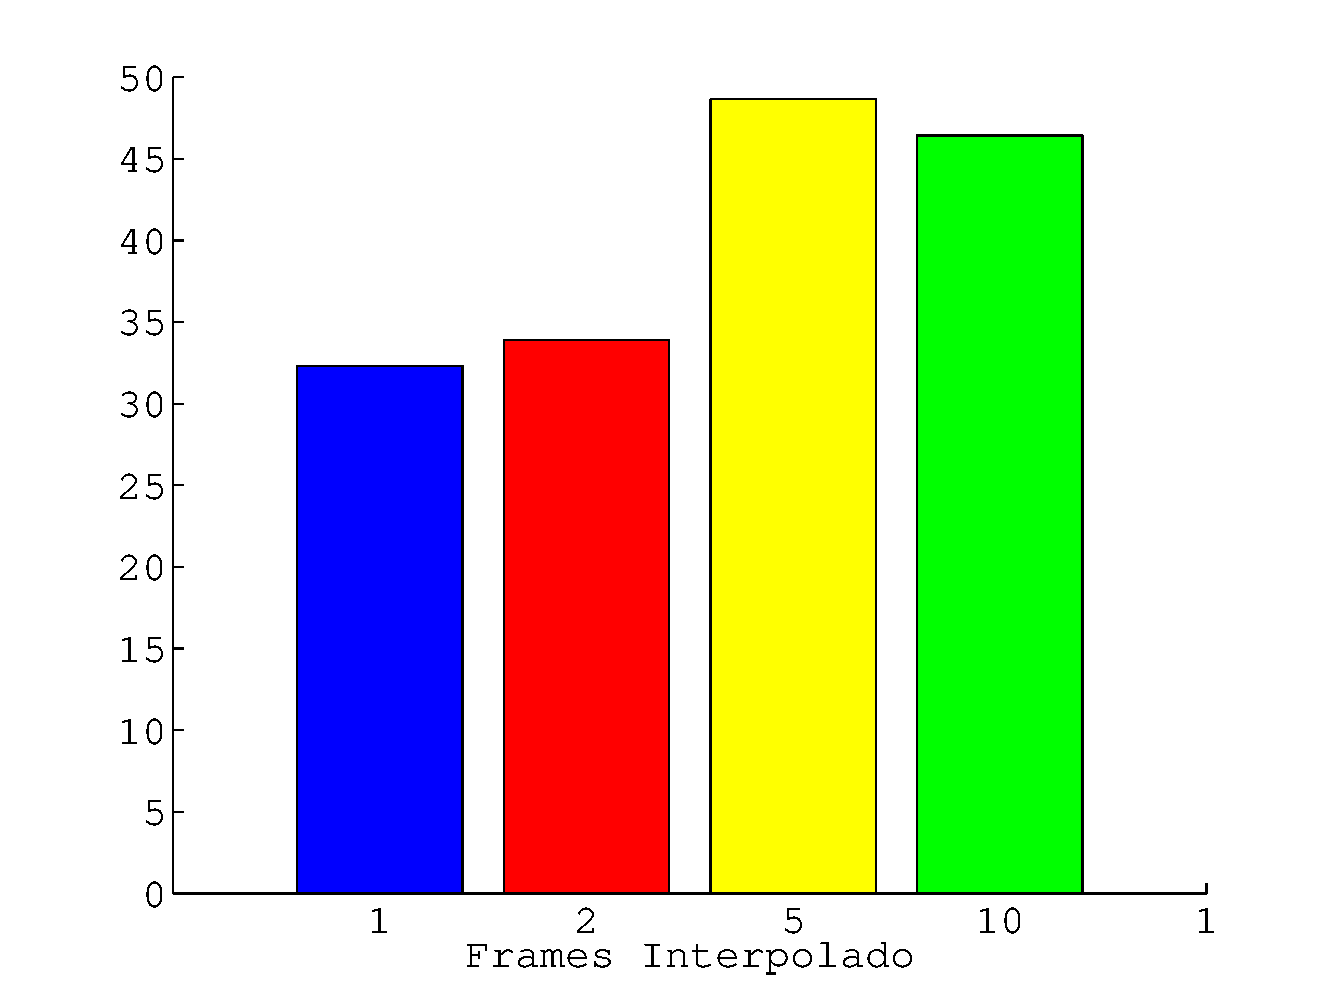
\includegraphics[width=.25\textwidth]{camara_fija-imagen_fija-max_vecino.pdf}
    }%\hspace{20pt}
    \subfloat[][M\'inimo]{
        \includegraphics[width=.25\textwidth]{camara_fija-imagen_fija-min_vecino.pdf}
    }
    \caption{Est\'adisticas ECM Seg\'un Frames Interpolados - M\'etodo Vecino M\'as Cercano}
    \label{fig:fija-fija_vecino-mse_estadisticas}
\end{figure}

\par En los resultados expuestos en la figura \ref{fig:fija-fija_vecino-mse_estadisticas}
se encuentran relaciones entre las distintas variantes de frames interpolados, y
con n\'umeros bastantes cercanos tambi\'en, que al caso de splines. La diferencia
destacable radica en los valores de error m\'inimo alcanzado para las variantes de
interpolaci\'on de 1 y 10 frames, que como se puede observar son mucho m\'as chicos
que para los par\'ametros restantes. A\'un as\'i, una vista detallada de los valores nominales
nos muestra que a pesar de ser estos muy peque\~nos, ya se est\'a teniendo errores
m\'inimos de valor nominal muy peque\~no, haciendo que esta diferencia entre
distintas variantes del m\'etodo sean poco importantes. Es decir, tanto como si
se interpolan 1, 2, 5 o 10 frames, pareciera que siempre habr\'a alg\'un frame
interpolado con pr\'acticamente 0 error de estimaci\'on.

\par Respecto del an\'alisis del PSNR, y del video de comparaci\'on, los resultados
observados son exactamente id\'enticos a los explicados en el caso del m\'etodo
lineal para este video.

%\begin{figure}[H]
%    \centering
%    \includegraphics[width=.85\textwidth]{camara_fija-imagen_fija-vecino-psnr-k1.pdf}
%    \caption{PSNR para 1 frame interpolado - M\'etodo Vecino M\'as Cercano}
%    \label{fig:fija-fija_vecnio-psnr-k1}
%\end{figure}

%\begin{figure}[H]
%    \centering
%    \includegraphics[width=\textwidth]{camara_fija-imagen_fija-vecino-k10.png}
%    \label{fig:fija-fija_vecino-heatmap}
%    \caption{Regi\'on peor aproximada por la interpolaci\'on del vecino m\'as cercano}
%\end{figure}

%---------------------------------------------------------------
\subsubsection{An\'alisis entre M\'etodos}
\par Luego de haber analizado cada m\'etodo independientemente de los dem\'as,
bas\'andonos \'unicamente en sus par\'ametros, pasamos a comparar cada m\'etodo
cualitativamente respecto de los otros, siempre para el mismo video.

\par En la figura \ref{fig:fija-fija_metodos} se puede observar el ECM y PSNR
frame a frame para el caso de 2 frames interpolados de c\'ada uno de los
m\'etodos.  En el caso del m\'etodo de splines, se expuso los resultados para
la interpolaci\'on del video completo (sin dividir por bloques), ya que como se
vi\'o en su respectivo an\'alisis, el comportamiento era similar no importa el
tama\~no del bloque.

\begin{figure}[H]
    \centering
    \subfloat[][ECM para 2 frames interpolados]{
        \includegraphics[width=.5\textwidth]{mse_methods-camara_fija-imagen_fija-k2.pdf}
        \label{subfig:fija-fija_mse-k2}
    }
    \subfloat[][PSNR para 2 frames interpolados]{
        \includegraphics[width=.5\textwidth]{psnr_methods-camara_fija-imagen_fija-k2.pdf}
        \label{subfig:fija-fija_psnr-k2}
    }
    \caption{Comparativa de m\'etodos para 2 frames interpolados}
    \label{fig:fija-fija_metodos}
\end{figure}

\par En ambos gr\'aficos (aunque m\'as claramente en el PSNR) se observa un patr\'on
claro (m\'as all\'a de que haya frames que sean excepciones): la fidelidad es mejor
(o el error es menor) para el m\'etodo del vecino m\'as cercano, seguido por la
interpolaci\'on lineal y por \'ultimo el m\'etodo de splines.

\par No se exponen estas comparativas para otras variantes de interpolaci\'on,
ya que este patr\'on se repite en todos los casos. Adem\'as, vale la pena
recordar que para la cantidad de frames interpolados igual a 2 es para el cual
se obten\'ia el menor ECM medio para los m\'etodos de splines y vecino, y
virtualmente el menor tambi\'en para la interpolaci\'on lineal (la diferencia
para frames interpolados igual a 1 es m\'inima).

\par Pasemos a observar a continuaci\'on, las comparaciones para los valores
estad\'isticos del error cuadr\'atico medio:

\begin{figure}[H]
    \centering
    \subfloat[][Valor Medio]{
        \includegraphics[width=.5\textwidth]{mean_methods-camara_fija-imagen_fija.pdf}
    }
    \subfloat[][Desv\'io Est\'andar]{
        \includegraphics[width=.5\textwidth]{std_methods-camara_fija-imagen_fija.pdf}
    }\\
    \subfloat[][M\'aximo]{
        \includegraphics[width=.5\textwidth]{max_methods-camara_fija-imagen_fija.pdf}
    }
    \subfloat[][M\'inimo]{
        \includegraphics[width=.5\textwidth]{min_methods-camara_fija-imagen_fija.pdf}
    }
    \caption{Est\'adisticas ECM - Comparativa de M\'etodos}
    \label{fig:fija-fija_methods-mse_estadisticas}
\end{figure}

\par Al observarse estos datos, aparece algo que \emph{a priori} parecer\'ia
una contradicci\'on: el valor medio del ECM para el m\'etodo lineal es menor en
2 de las variantes (cantidad de frames 1 y 10) que el m\'etodo del vecino m\'as
cercano. Analizando un poco esto (pues, como afirmamos unos p\'arrafos m\'as
arriba, para todas las variantes encontramos que el PSNR para el m\'etodo del
vecino m\'as cercano segu\'ia el patr\'o de ser m\'as alto que el de los
restantes m\'etodos), entendemos que el motivo de esto se debe a que el
m\'etodo del vecino tiene picos m\'as amplios donde comete mucho m\'as error
que el m\'etodo de interpolaci\'on lineal. Esto puede observarse, nuevamente,
en la figura \ref{fig:fija-fija_metodos}.  Esto explica el porque del valor
medio del error es m\'as bajo para el m\'etodo lineal, aunque en la gran
mayor\'ia de los frames la aproximaci\'on del m\'etodo del vecino es mejor.

%---------------------------------------------------------------
\subsubsection{Conclusiones}
\par A lo largo de la experimentaci\'on para el tipo de video
\emph{c\'amara-fija, im\'agen fija}, observamos que todos los m\'etodos
mostraron un buen comportamiento.  Esta afirmaci\'on es subjetiva y basada en
la opini\'on de los autores luego de observar los videos resultantes. Para el
ojo humano, las diferencias entre los m\'etodos (o para el mismo m\'etodo con
diferentes par\'ametros) fueron imperceptibles.

\par A\'un as\'i, un an\'alisis m\'as objetivo basado en las m\'etricas nos
lleg\'o a indicar que, al menos para los par\'ametros evaluados, el m\'etodo
del vecino pareciera ser mejor, incluso cuando se interpolan muchos frames
(recordemos que una las hip\'otesis al comienzo de la experimentaci\'on era que
los m\'etodos de spline e interpolaci\'on lineal deber\'ian ser mejores en caso
de tener que estimar/reconstruir muchos frames). Si bien su ECM medio es m\'as
alto que el de otros m\'etodos, pudimos observar que tambi\'en lo es su
desv\'io est\'andar. Y justamente esto \'ultimo es lo que nos permiti\'o
descubrir que el motivo de su ECM medio m\'as alto se debe a que, en
determinados frames (los m\'as alejados de los 2 frames utilizados para
interpolar, de hecho) el m\'etodo tiene un error m\'as alto que el resto. Como
esto \'ultimo ocurre seguido, el ECM tiende a subir, pero al observar el PSNR
frame a frame se pudo concluir que en realidad, para la gran mayor\'ia de los
frames interpolados, el m\'etodo del vecino superaba a sus pares.

\par Esto \'ultimo no es un resultado menor, m\'as si se tiene en cuenta que
el m\'etodo del vecino es el m\'as barato computacionalmente hablando, como ya
se ha visto.

\par En otra l\'inea de an\'alisis, tambi\'en se observ\'o que al menos para
este tipo de video, que el tama\~no de bloque utilizado no hizo variar a la
efectividad del m\'etodo de spline. Esto, si bien no esperado al comenzar los
experimentos, es razonable si se considera que en si mismo el video no presenta
casi cambios, m\'as all\'a del brillo de sus puntos debido al cambio de
iluminaci\'on. Tiene sentido entonces que el resultado de splines no var\'ie ya
que ''la funci\'on interpolada''\footnote{Los pixels a lo largo de los frames.}
camb\'ian en funci\'on del frame de manera ''suave'', con lo cual no importe
desde que frame a que frame se genere el spline, sus valores en los extremos de
los bloques tender\'ian a ser similiares a lo que se les exije en el m\'etodo a
los \emph{sub-splines}.

\par Para finalizar este experimento, vale la pena remarcar nuevamente que si
bien la interpolaci\'on de todos los m\'etodos tuvieron error, el mismo siempre
fue muy peque\~no nominalmente. De hecho, como se mencion\'o al principio de
estas conclusiones, fueron imperceptibles para los autores. Si se observan los
errores m\'aximos obtenidos de todos los m\'etodos, observamos que el error
m\'as grosero cometido fue de 60, el cual quedar\'a en evidencia que es un
valor peque\~no al compararlo con los errores de los m\'etodos en los otros
tipos de videos que se exponen m\'as adelante. M\'as a\'un, si se observar los
videos comparativos de las interpolaciones, se observar\'a que el \emph{heatmap}
de la diferencia absoluta entre el frame original y el interpolado nunca tiene
regiones enteras con mucho (o incluso, m\'as que poco) error. A lo sumo existen
peque\~nos grupos de no m\'as de 10 p\'ixeles que muestran un error alto, pero
nunca regiones.

%---------------------------------------------------------------


%---------------------------------------------------------------
\newpage
\subsection{C\'amara Fija - Im\'agen M\'ovil}
\IEEEPARstart{H}{abiendo} ya realizado detalladamente el an\'alsis propuesto
por la metdolog\'ia explicada en la secci\'on~\ref{subsec:metodologia} para
el caso de \emph{c\'amara fija, im\'agen fija} (secci\'on
\ref{subsec:fija-fija}), no ahondaremos tanto en detalles sobre la explicaci\'on
de los datos obtenidos. Los gr\'aficos, tablas e histogramas utilizados son los
mismos para este caso y los que le siguen\footnote{C\'amara m\'ovil, im\'agen
fija y m\'ovil.}. Simplemente expondremos los resultados y los analizaremos.

%---------------------------------------------------------------
\subsubsection{Spline}

\begin{figure}[H]
    \centering
    \subfloat[][ECM para 1 frames interpolados]{
        \includegraphics[width=.5\textwidth]{mse_spline-camara_fija-imagen_movil-k1.pdf}
        \label{subfig:fija-movil_spline-mse-k1}
    }
    \subfloat[][ECM para 10 frames interpolados]{
        \includegraphics[width=.5\textwidth]{mse_spline-camara_fija-imagen_movil-k10.pdf}
        \label{subfig:fija-movil_spline-mse-k10}
    }\\
    \subfloat[][PSNR para 1 frames interpolados]{
        \includegraphics[width=.5\textwidth]{psnr_spline-camara_fija-imagen_movil-k1.pdf}
        \label{subfig:fija-movil_spline-psnr-k1}
    }
    \subfloat[][PSNR para 10 frames interpolados]{
        \includegraphics[width=.5\textwidth]{psnr_spline-camara_fija-imagen_movil-k10.pdf}
        \label{subfig:fija-movil_spline-psnr-k10}
    }
    \caption{Comparativa tama\~no de bloque para 1 y 10 frames interpolados}
    \label{fig:fija-movil_spline-mse-bloques}
\end{figure}

\par En primer lugar, al igual que para el experimento previo, se exponen
s\'olo los gr\'aficos comparativos de tama\~no de bloque del ECM por frame para
1 y 10 frames interpolados (figura \ref{fig:fija-movil_spline-mse-bloques}). No
se exponen los casos para 2 y 5 frames interpolados ya que el comportamiento
observado se refleja de la misma manera en estos, y para explicar el mismo
alcanza con las variantes expuestas.

\par Lo que se observa inicialmente de la figura
\ref{subfig:fija-movil_spline-mse-k1} respecto del tama\~no de bloque, es que
para este video el tama\~no de bloque 4 pareciera ser significativamente
mejor\footnote{Menos error.} que para los dem\'as tama\~nos (m\'as all\'a de
algunos pocos frames donde esto no ocurre). M\'as a\'un, en t\'erminos generales
m\'as all\'a de frames excepcionales, se observa que el ECM aumenta a medida que
aumenta el tama\~no de bloque.

\par Sin embargo, esto no pareciera ser tan claro para el caso de 10 frames
interpolados (figura \ref{subfig:fija-movil_spline-mse-k10}). En \'este se puede
distinguir que el tama\~no de bloque 4 suele tener menos error que el resto de
los tama\~nos, aunque la diferencia es notoriamente menor que para el caso de
1 frame interpolado. Y, \'aun m\'as, no queda claro a simple vista que el error
vaya aumentando a medida que aumenta el tama\~no de bloque (solapamiento de los
ECM), aunque s\'i podemos afirmar que la interpolaci\'on por spline para todo
el video (sin dividir en bloques) es el que suele tener para la gran mayor\'ia
de los frames el ECM m\'as alto. Este solapamiento no queda del todo claro en
esta figura, principalmente dado que la escala difiere respecto de la figura
\ref{subfig:fija-movil_spline-mse-k1}, pero queda ya claro al observar los
gr\'aficos de PSNR, que tienen la particularidad de normalizar respecto del
valor m\'aximo de los p\'ixeles los valores del ECM.

\par M\'as a\'un, si tenemos en cuenta el ECM/PSNR para 2 y 5 frames interpolados,
el patr\'on que se observa es que a medida que se interpolan m\'as frames se
incrementa el solapamiento, es decir, se ''pegan'' las funciones de ECM para
los distintos tama\~nos de bloque. Aunque, como parte de este patr\'on, pareciera
que a menor tama\~no de bloque se sigue comientiendo menos error.

\par B\'asicamente, se observa un patr\'on: a menor tama\~no de bloque menor
error cometido, aunque esta diferencia a favor de una interpolaci\'on de menor
tama\~no de bloque se va diluyendo a medida que se incrementa la cantidad de
frames interpolados.

\par Si nos detenemos en los cuadros de la figura
\ref{fig:fija-movil-dif_ecm_splines}, se observar\'a que se confirm\'a este
patr\'on\footnote{A modo de recordatorio, cada cuadro nos indica la diferencia
m\'axima del error para un mismo frame interpolado. B\'asicamente, en la
posici\'on $i,j$, tendremos la diferencia m\'axima de las estimaciones sobre
las cuales el tama\~no de bloque $i$ cometi\'o un error mayor que tama\~no
$j$.}. Se puede observar aqu\'i que para cualesquiera 2 tama\~nos de bloque
distintos, la m\'axima diferencia del ECM para un mismo frame siempre es mayor
para el tama\~no de bloque mayor. Por ejemplo, si tomamos los tama\~nos 4 y 8,
veremos que siempre 4 vs 8 (la diferencia m\'axima para la cual el ECM de 4 es
mayor al de 8) es mayor a 8 vs 4.

\begin{figure}[H]
    \centering
    \subfloat[][1 Frame Interpolado]{
        \footnotesize
        \setlength{\tabcolsep}{3pt}
        \begin{tabular}{|l|r|r|r|r|r|}
            \hline
            \textbf{Bloque}& \textbf{vs 4}& \textbf{vs 8}& \textbf{vs 16}& \textbf{vs 32}& \textbf{vs Entero}\\
            \hline\hline
            \textbf{4}&0& 1.0553& 1.3580& 1.5157& 0.0836\\
            \textbf{8}&2.2855& 0& 1.3654& 1.4776& 0.5794\\
            \textbf{16}&2.4014& 1.8014& 0& 0.3766& 0.0696\\
            \textbf{32}&2.5348& 1.8834& 1.4168& 0& 0.6421\\
            \textbf{Entero}&2.5429& 1.9027& 1.5443& 1.5157& 0\\
            \hline
        \end{tabular}
    }\hspace{10pt}
    \subfloat[][2 Frames Interpolados]{
        \footnotesize
        \setlength{\tabcolsep}{3pt}
        \begin{tabular}{|l|r|r|r|r|r|}
            \hline
            \textbf{Bloque}& \textbf{vs 4}& \textbf{vs 8}& \textbf{vs 16}& \textbf{vs 32}& \textbf{vs Entero}\\
            \hline\hline
            \textbf{4}&0& 1.0587& 1.4019& 1.5831& 0.5797\\
            \textbf{8}&2.6425& 0& 1.1953& 1.4636& 0.7106\\
            \textbf{16}&2.7262& 1.6141& 0& 0.3542& 0.0415\\
            \textbf{32}&2.7816& 1.7799& 1.3980& 0& 0.0566\\
            \textbf{Entero}&2.7875& 1.7952& 1.4049& 1.5831& 0\\
            \hline
        \end{tabular}
    }\\
    \subfloat[][5 Frames Interpolados]{
        \footnotesize
        \setlength{\tabcolsep}{3pt}
        \begin{tabular}{|l|r|r|r|r|r|}
            \hline
            \textbf{Bloque}& \textbf{vs 4}& \textbf{vs 8}& \textbf{vs 16}& \textbf{vs 32}& \textbf{vs Entero}\\
            \hline\hline
            \textbf{4}&0& 0.8709& 0.6384& 1.8067& 0.6342\\
            \textbf{8}&3.4411& 0& 0.6755& 1.6095& 0.6634\\
            \textbf{16}&3.5990& 3.2710& 0& 1.4143& 0.1297\\
            \textbf{32}&3.6145& 3.3025& 0.9938& 0& 0.0607\\
            \textbf{Entero}&3.6162& 3.3024& 1.0310& 1.8448& 0\\
            \hline
        \end{tabular}
    }\hspace{10pt}
    \subfloat[][10 Frames Interpolados]{
        \footnotesize
        \setlength{\tabcolsep}{3pt}
        \begin{tabular}{|l|r|r|r|r|r|}
            \hline
            \textbf{Bloque}& \textbf{vs 4}& \textbf{vs 8}& \textbf{vs 16}& \textbf{vs 32}& \textbf{vs Entero}\\
            \hline\hline
            \textbf{4}&0& 1.5891& 0.8529& 0.6327& 0.5407\\
            \textbf{8}&3.2999& 0& 1.5430& 0.7919& 0.7928\\
            \textbf{16}&3.6673& 2.3288& 0& 0.5000& 0.5016\\
            \textbf{32}&3.8571& 3.0513& 2.4365& 0& 0.2676\\
            \textbf{Entero}&3.8574& 3.0504& 2.4367& 0.6565& 0\\
            \hline
        \end{tabular}
    }
    \caption{Diferencia m\'axima de ECM para mismo frame seg\'un tama\~no de bloque}
    \label{fig:fija-movil-dif_ecm_splines}
\end{figure}


\par Ahora bien, siguiendo esta l\'inea de an\'alisis, se observa (salvo alguna
excepci\'on) otro patr\'on: a medida que se interpolan m\'as frames, las
diferencias m\'aximas del ECM incrementarse para los casos de tama\~no $i$ vs
$j$ con $i>j$, y decrementarse para $i<j$. Es decir, mientras que en el
gr\'afico \ref{subfig:fija-movil_spline-psnr-k10} se observa un mayor
solapamiento del PSNR, en las tablas de la figura
\ref{fig:fija-movil-dif_ecm_splines} vemos que las diferencias m\'aximas (o
picos) entre dos interpolaciones con distinto tama\~no de bloque se incrementan
a mayor cantidad de frames interpolados. Es decir, si bien en la media los
tama\~nos de bloque est\'an cada vez m\'as cerca a mayor cantidad de frames
interpolados, los errores m\'aximos cometidos por las interpolaciones con mayor
tama\~no de bloque respecto de los de menor tama\~no se incrementan (es decir,
mayores picos de error entre distintos tama\~nos\footnote{A no confundir con
los picos de error absoluto. Aqu\'i nos referimos a los errores m\'aximos entre
dos interpolaciones de la misma cantidad de frames pero distinto tama\~no se
incrementa a mayor cantidad de frames interpolados.}).

\begin{figure}[H]
    \centering
    \subfloat[][Valor Medio]{
        \includegraphics[width=.5\textwidth]{camara_fija-imagen_movil-mean_spline.pdf}
    }
    \subfloat[][Desv\'io Est\'andar]{
        \includegraphics[width=.5\textwidth]{camara_fija-imagen_movil-std_spline.pdf}
    }\\
    \subfloat[][M\'aximo]{
        \includegraphics[width=.5\textwidth]{camara_fija-imagen_movil-max_spline.pdf}
    }
    \subfloat[][M\'inimo]{
        \includegraphics[width=.5\textwidth]{camara_fija-imagen_movil-min_spline.pdf}
    }
    \caption{Est\'adisticas ECM Seg\'un Frames Interpolados - Spline}
    \label{fig:fija-movil_spline-mse_estadisticas}
\end{figure}

\par En las estad\'isticas expuestas en la figura
\ref{fig:fija-movil_spline-mse_estadisticas} se observa otra confirmaci\'on del
patr\'on mencionado. Se puede ver que la media del ECM para una misma cantidad
de frames interpolados (barras del mismo color) es menor a menor tama\~no de
bloque (aunque las diferencias no son tan significativas entre tama\~nos
consecutivos). Y tambi\'en se observa que esta media es menor a menor cantidad
de frames interpolados, lo que es consistente con nuestras hip\'otesis
iniciales.

\par Tambi\'en observamos que este patr\'on se mantiene en el caso del desv\'io
est\'andar de los datos. Es decir, hay una varianza menor para a menor cantidad
de frames interpolados, y ligeramente menor para una misma cantidad de frames
interpolados pero con tama\~nos de bloque menores.

\par Otra cosa que destaca de la figura \ref{fig:fija-movil_spline-mse-bloques}
es que se observa una mayor cantidad de errores (o menor PSNR) en los primeros
frames (el primer cuarto de video). Analizando el video
comparativo\footnote{\url{https://drive.google.com/open?id=0B0RfkWV-4-XqSHJ3NXBSRUo4SjQ}}
de las diferencias entre frames originales e interpolados para tama\~no de
bloque 4 (menor ECM medio) y 10 frames interpolados (mayor varianza dentro de
las variantes de cantidad de frames interpolados)\footnote{La elecci\'on de
estos par\'ametros para le generaci\'on del video de diferencias frame a frame
se basa en los mismos argumentos que en el caso de splines del experimento
previo.}, observamos que al comienzo del video (una jugada de un partido de
f\'utbol desde un punto fijo) tenemos un jugador que comienza a correr en un
primer plano, mientras que el resto de los jugadores en movimiento se
encuentran en un plano cada vez m\'as lejano. En la figura
\ref{fig:fija-movil_spline-heatmap} se observa una captura del video comparador
representativo de esto.

\begin{figure}[H]
    \centering
    \includegraphics[width=\textwidth]{camara_fija-imagen_movil-spline-k10-blk4.png}
    \label{fig:fija-movil_spline-heatmap}
    \caption{Regi\'on peor aproximada por la interpolaci\'on por spline}
\end{figure}

\par En el video comparador queda claro que los movimientos de los jugadores
son los que m\'as error aportan a la interpolaci\'on. Y no s\'olo eso, sino que
el hecho de que haya jugadores en planos m\'as cercanos a la c\'amara generan
un mayor error en la interpolaci\'on, ya que dichos jugadores ''ocupan'' una
mayor cantidad de pixeles de los frames que aquellos que se encuentran en
planos m\'as lejanos. Este jugador que comienza en un plano m\'as cercano, al
comenzar a pasar a planos cada vez m\'as lejanos comienza a ser representado por
cada vez menos p\'ixeles, y as\'i entonces cada vez disminuye su injerencia
en el error de la interpolaci\'on (menos pixeles interpolados con cambios debidos
al desplazamiento de este jugador). Y esto queda evidenciado en las primeras
figuras donde observamos que en el \'ultimo cuarto de video/frames los picos del
ECM son menores (o que los del PSNR son cada vez mayores).

%---------------------------------------------------------------
\subsubsection{Interpolaci\'on Lineal}

\begin{figure}[H]
    \centering
    \subfloat[][Valor Medio]{
        \includegraphics[width=.25\textwidth]{camara_fija-imagen_movil-mean_lineal.pdf}
    }
    \subfloat[][Desv\'io Est\'andar]{
        \includegraphics[width=.25\textwidth]{camara_fija-imagen_movil-std_lineal.pdf}
    }
    \subfloat[][M\'aximo]{
        \includegraphics[width=.25\textwidth]{camara_fija-imagen_movil-max_lineal.pdf}
    }
    \subfloat[][M\'inimo]{
        \includegraphics[width=.25\textwidth]{camara_fija-imagen_movil-min_lineal.pdf}
    }
    \caption{Est\'adisticas ECM Seg\'un Frames Interpolados - M\'etodo Lineal}
    \label{fig:fija-movil_lineal-mse_estadisticas}
\end{figure}

\par Observando las est\'adisticas del m\'etodo para las distintas variantes
de la cantidad de frames interpolados, se hayan resultados que son consistentes
con las hip\'otesis iniciales enunciadas. Se observa como el ECM medio es cada
vez mayor a medida que se interpolan m\'as frames (es decir, se utilizan 2 frames
para interpolar una cantidad cada vez mayor de frames entre ambos).

\par Adem\'as tambi\'en se observa que la varianza del error de la
aproximaci\'on de la interpolaci\'on aumenta conforme aumenta la cantidad de
frames interpolados (lo cual es de alguna manera razonable, al interpolarse
m\'as frames, los frames interpolados m\'as cercanos a los frames utilizados en
la interpolaci\'on tendr\'an menor error, mientras que a mayor distancia de
estos m\'as error habr\'a, generando multiples valores de error distintos y
distantes entre s\'i -y de la media-). Este \'ultimo comportamiento se puede
observar m\'as claramente en la figura \ref{fig:fija-movil_lineal-psnr-k10}.

\begin{figure}
    \centering
    \includegraphics[width=.85\textwidth]{camara_fija-imagen_movil-lineal-psnr-k10.pdf}
    \caption{PSNR para 10 frames interpolados - M\'etodo Lineal}
    \label{fig:fija-movil_lineal-psnr-k10}
\end{figure}

\par Aqu\'i se puede observar como el PSNR\footnote{Recordemos que el PSNR, a
diferencia del ECM, nos da una noci\'on de la calidad de la estimaci\'on del
frame. Es decir, a mayor PSNR, menor ECM (aunque la relaci\'on no es lineal, ya
que el PSNR normaliza la medida seg\'un el valor m\'aximo de los p\'ixeles).}
tiene un comportamiento oscilante, yendo de un valor ''alto'' de PSNR a uno
bajo y luego comenzando a ascender nuevamente hasta llegar a otro pico ''alto''.

\par De la observaci\'on se determin\'o que estos picos ''altos'' son los frames
interpolados inmediatos a los frames originales utilizados para calclular la
funcion interpoladora, y no es coincidencia que los picos ''bajos'' (donde hay
mayor error en la interpolaci\'on) sean justamente los frames intermedios entre
dos frames utilizados para calcular el polinomio interpolador lineal.

\par Pasando a analizar el video comparador para 10 frames
interpolados\footnote{\url{https://drive.google.com/open?id=0B0RfkWV-4-XqMHNrY3JqVHlOUXc}},
observamos el mismo comportamiento visto para el caso de splines, aunque los
errores cometidos para las reginoes con poco (o ning\'un) movimiento
parecer\'ian ser menores que para splines. En todo caso, esto se estudiar\'a al
final de esta secci\'on al comparar los distintos m\'etodos entre s\'i.

%---------------------------------------------------------------
\subsubsection{Vecino m\'as Cercano}

\begin{figure}[H]
    \centering
    \subfloat[][Valor Medio]{
        \includegraphics[width=.25\textwidth]{camara_fija-imagen_movil-mean_vecino.pdf}
    }
    \subfloat[][Desv\'io Est\'andar]{
        \includegraphics[width=.25\textwidth]{camara_fija-imagen_movil-std_vecino.pdf}
    }
    \subfloat[][M\'aximo]{
        \includegraphics[width=.25\textwidth]{camara_fija-imagen_movil-max_vecino.pdf}
    }
    \subfloat[][M\'inimo]{
        \includegraphics[width=.25\textwidth]{camara_fija-imagen_movil-min_vecino.pdf}
    }
    \caption{Est\'adisticas ECM Seg\'un Frames Interpolados - M\'etodo Vecino M\'as Cercano}
    \label{fig:fija-movil_vecino-mse_estadisticas}
\end{figure}

\par Nuevamente, para este m\'etodo y este video, encontramos resultados
consistentes con nuestras hip\'otesis. A mayor cantidad de frames interpolados,
mayor es el error medio. De hecho, los resultados de este m\'etodo son muy
similares a los de la interpolaci\'on lineal (en cuanto a la relaci\'on del
mismo m\'etodo para distintos frames interpolados, no en cuanto a los valores
de ECM de vecino m\'as cercano contra interpolaci\'on lineal). Aunque, salta a
la vista que el desv\'io est\'andar para la interpolaci\'on de 2 frames es
ligeramente menor que para la de 1 frame.

\par Voliendo sobre los conceptos del m\'etodo, es de alguna manera razonable
explicar esto debido a que al tener 2 frames interpolados por cada par
consecutivo de frames del video original, cada uno de los interpolados ser\'a
una copia exacta de su frame original m\'as cercano. De esta manera, deber\'ian
haber movimientos/cambios muy bruscos en los frames originales (como por
ejemplo, un cambio de c\'amara si se estuviera trabajando con el video de una
transimici\'on de televisi\'on o una pel\'icula) de manera que el frame
copiado/interpolado fuera completamente distinto al frame original al que
deber\'ia aproximar. Dado que esto no ocurre en nuestro video, es razonable
pensar que la diferencia de un frame a otro no tenga grandes diferencias, de
manera que al utilizar una copia del vecino m\'as cercano para una
interpolaci\'on de pocos frames no tenga demasiado error ni mucha varianza (ya
que el error de todos los frames interpolados/copiados es la diferencia de 2
frames consecutivos del video original, los cuales para un video sin cambios
bruscos deberia ser similar para todos los frames).

\par Analizando el video comparativo para este
m\'etodo\footnote{\url{https://drive.google.com/open?id=0B0RfkWV-4-XqY1gtZDFqQ0puaTg}},
adem\'as de observar el mismo comportamiento respecto de los movimientos/planos
donde se genera el error en la interpolaci\'on, observamos que hay saltos entre
frames donde el error aparece ''repentinamente''. Obviamente esto se debe a el
cambio de un frame a otro sin ning\'un intento de aproximar lo que ocurre en el
medio. Esto no ocurr\'ia para el experimento previo, ya que ahora tenemos
movimientos cuando antes s\'olo teniamos cambios de luz/tonalidad. Si bien no
podemos exponer en este documento en forma de gr\'afico esta percepci\'on, si
podemos presentar el gr\'afico del PSNR frame a frame, donde se puede observar
los picos de muy pronunciados de p\'erdida de precisi\'on (o aumento del error)
que ocurren de manera c\'iclica (con esto nos refer\'imos a que ocurren a un
intervalo regular de frames, no a que su valor PSNR sea el mismo).

\begin{figure}
    \centering
    \includegraphics[width=.85\textwidth]{camara_fija-imagen_movil-vecino-psnr-k10.pdf}
    \caption{PSNR para 10 frames interpolados - Vecino m\'as Cercano}
    \label{fig:fija-movil_vecino-psnr-k10}
\end{figure}

\par Aqu\'i lo que se nota de distinto respecto de los otros m\'etodos, que por
ah\'i no es tanto el intervalo de los picos de error (bajo PSNR), es el hecho
de que los mismos son abruptos (pasan de un PSNR alto a un PSNR bajo de manera
muy r\'apida), mientras que en los casos anteriores observamos como estos cambios
se dan de forma m\'as ''suave'': es decir, graficamente hablando, de una manera
no tan ''recta'' sino m\'as curva (ver figura \ref{fig:fija-movil_lineal-psnr-k10}).

%---------------------------------------------------------------
\subsubsection{An\'alisis entre M\'etodos}

\begin{figure}[H]
    \centering
    \subfloat[][PSNR para 1 frames interpolados]{
        \includegraphics[width=.5\textwidth]{psnr_methods-camara_fija-imagen_movil-k1.pdf}
        \label{subfig:fija-movil_psnr-k1}
    }
    \subfloat[][PSNR para 2 frames interpolados]{
        \includegraphics[width=.5\textwidth]{psnr_methods-camara_fija-imagen_movil-k2.pdf}
        \label{subfig:fija-movil_psnr-k2}
    }\\
    \subfloat[][PSNR para 5 frames interpolados]{
        \includegraphics[width=.5\textwidth]{psnr_methods-camara_fija-imagen_movil-k5.pdf}
        \label{subfig:fija-movil_psnr-k5}
    }
    \subfloat[][PSNR para 10 frames interpolados]{
        \includegraphics[width=.5\textwidth]{psnr_methods-camara_fija-imagen_movil-k10.pdf}
        \label{subfig:fija-movil_psnr-k10}
    }
    \caption{Comparativa de m\'etodos}
    \label{fig:fija-movil_metodos}
\end{figure}

\par En la figura \ref{fig:fija-movil_metodos} se presentan el PSNR para las
distintas variantes de cantidad de frames interpolados, comparando los m\'etodos
que objeto de estudio de este trabajo. En el caso particular del m\'etodo de
spline, se tom\'o el tama\~no de bloque 4, habi\'endose visto que este era el
que menor error presentaba para cualquiera de las variantes de cantidad de frames
interpodos.

\par Para todos las variantes expuestas, el primer resultado obvio es que
spline parecier\'a ser el m\'etodo que pero estima los frames. Se observa que
para todos los frames interpolados, es siempre el m\'etodo de menor PSNR. Y,
como ya se ha visto, splines es el m\'etodo m\'as costoso de los 3 que est\'an
siendo estudiados, con lo cual este resultado ya nos permite proponer que a la
hora de utilizar este tipo de videos (c\'amara fija, im\'agen m\'ovil -sin
movimientos bruscos-) splines no parece ser un m\'etodo a ser
considerado\footnote{Quiz\'as si evalu\'asemos variantes donde se interpolen
una mayor cantidad de frames, estos resultados podr\'ian variar. Pero ya tener
una interpolaci\'on de 10 frames es considerable, sumado las limitantes de
tiempo para experimentar con valores m\'as altos.}.

\par Queda entonces evaluar que ocurre con los m\'etodos del vecino e
interpolaci\'on lineal. Observando las figuras \ref{subfig:fija-movil_psnr-k1}
y \ref{subfig:fija-movil_psnr-k2}, se ve que en la primera mitad del video el
PSNR de ambos m\'etodos es similar, para luego en la segunda mitad obtener la
interpolaci\'on lineal mejores resultados (en el caso de 2 frames interpolados,
esta ventaja es m\'inima y quiz\'as desestimable). En los casos restantes, es
claro que durante todo el video el m\'etodo del vecino estima de mejor manera
los frames reconstru\'idos. No es casualidad que, en los casos donde la
interpolaci\'on lineal supera al m\'etodo del vecino, se de justo en el momento
en que aparece un jugador en el primer plano del video (alrededor del frame
110). Pareciera que al interpolar pocos frames y haber movimiento en un \'area
considerable de los frames el m\'etodo lineal se comporta mejor que el resto.
Lo sorpresivo es, dadas nuestras hip\'otesis, que al aumentar la cantidad de
frames el PSNR sea mucho mejor para el metodo del vecino.

\par Si observamos las estad\'isticas del ECM de la figura 
\ref{fig:fija-movil_methods-mse_estadisticas}, veremos que los resultados
reflejan este mismo comportamiento (bien podr\'ia, debido a un desv\'io est\'andar
alto o una cantidad de \emph{outliers} suficiente, no hacerlo). Se observa que
para pocos frames el ECM medio del m\'etdo lineal es menor, y que a medida que
aumenta la cantidad de frames estimados el m\'etodo del vecino comienza a tener
un ECM medio m\'as bajo relativo a los otros dos m\'etodos. Incluso esto mismo
ocurre con el desv\'io est\'andar (aunque la diferencia relativa que va ''ganando''
el m\'etodo del vecino crece a menor ratio).

\begin{figure}[H]
    \centering
    \subfloat[][Valor Medio]{
        \includegraphics[width=.5\textwidth]{mean_methods-camara_fija-imagen_movil.pdf}
    }
    \subfloat[][Desv\'io Est\'andar]{
        \includegraphics[width=.5\textwidth]{std_methods-camara_fija-imagen_movil.pdf}
    }\\
    \subfloat[][M\'aximo]{
        \includegraphics[width=.5\textwidth]{max_methods-camara_fija-imagen_movil.pdf}
    }
    \subfloat[][M\'inimo]{
        \includegraphics[width=.5\textwidth]{min_methods-camara_fija-imagen_movil.pdf}
    }
    \caption{Est\'adisticas ECM - Comparativa de M\'etodos}
    \label{fig:fija-movil_methods-mse_estadisticas}
\end{figure}

\par Continuando el an\'alisis de estos datos, se ve que el ECM m\'inimo para
el m\'etodo del vecino se ve casi inalterado sin importar la cantidad de frames
que se interpolen. Esto tiene sentido pues dado un frame, su frame interpolado
inmediato en la reproducci\'on ser\'a siempre el mismo sin importar cuantos
otros frames se copien hasta ''llegar'' al siguiente frame
no-interpolado/original. Por otro lado, si vemos que el comportamiento de los
m\'etodos restantes comienza cada vez a tener una peor cota para el frame mejor
aproximado a medida que se estima una mayor cantidad de frames. Claramente
estos m\'etodos son mucho m\'as sensibles a la ''distancia'' entre los frames
originales utilizados para calcular su polinomio interpolador\footnote{Recordar
que en nuestra experimentaci\'on se est\'a tomando un video y se le remueven
frames que luego ser\'an reconstru\'idos mediante los m\'etodos estudiados.}.

\par En cuanto al frame peor estimado (m\'aximo ECM) observamos que todas las
t\'ecnicas evaluadas comienzan a tener un frame cada vez peor aproximado. Esto,
de hecho, tiene sentido, ya que a medida que se incrementa la cantidad de
frames interpolados se deben generar artificialmente m\'as cuadros con menos
informaci\'on (frames originales m\'as ''distantes'' en la reproducci\'on del
video original). Claramente aproximar con menos informaci\'on reduce las
posibilidades de estimar de manera precisa.

\par Por \'ultimo, y para finalizar este an\'alisis de los m\'etodos para este
video, observamos los videos comparadores de utilizados en los an\'alisis
independientes de los m\'etodos para este video. A modo de presentar un resultado
en este trabajo, presentamos en la figura \ref{fig:fija-movil_heatmap} 3
capturas del mismo frame, que fue interpolado por los 3 m\'etodos.

\begin{figure}[H]
    \centering
    \subfloat[][Spline (tama\~no de bloque 4)]{
        \includegraphics[width=\textwidth]{camara_fija-imagen_movil-spline-k10-blk4.png}
    }\\
    \subfloat[][Interpolaci\'on Lineal]{
        \includegraphics[width=\textwidth]{camara_fija-imagen_movil-lineal-k10.png}
    }\\
    \subfloat[][Vecino m\'as Cercano]{
        \includegraphics[width=\textwidth]{camara_fija-imagen_movil-vecino-k10.png}
    }
    \caption{Captura del mismo frame de Videos comparativos para interpolaci\'on de 10 frames}
    \label{fig:fija-movil_heatmap}
\end{figure}

\par Como se puede observar en las figuras (o en los videos, cuyos \emph{links}
pueden encontrarse en las secciones previas) se ve que el movimiento de los
jugarores es el principal \'area de los frames que son estimados de la manera
menos precisa por cualquiera de los m\'etodos. Lo intersante es obsevar las
\'areas de los frames que no presentan movimientos (o que son imperceptibles o
claramente de menor intensidad que los pertenecientes a los jugadores). As\'i
se puede observar que el m\'etodo de splines comete errores peque\~nos a lo largo
de todo el cuadro, mientras que el m\'etodo lineal lo hace en menor medida y el
vecino m\'as cercano a\'un menos.

\par Esto nos explica, probablemente, porque el m\'etodo del vecino tiene un
ECM menor que los otros dos m\'etodos (o PSNR m\'as alto). Observando las tonalidades
de los errores de los jugadores, y el \'area que ocupan en el frame estos puntos
\textbf{negros}, observamos que los m\'etodos cometen errores similares a la hora
de estimar a los mismos. Por lo tanto, queda claro que es la estimaci\'on del
resto del frame que hace que un m\'etodo tenga menor error que otro.

\par El porque de este comportamiento podr\'ia explicarse dado que el m\'etodo
del vecino es m\'as ''bobo'' (aunque en este caso pareciera ser una ventaja), ya
que no asume nada sobre los pixeles y solo los copia. De esta manera, al tener
una gran parte de los cuadros del video que son est\'aticos (o con poqu\'isimo
movimiento) y no llegan a tener cambios de iluminaci\'on (como en el caso del
experimento previo), logra replicar este estatismo. Los m\'etodos restantes
tratan a cada pixel como una funci\'on a ser interpolada, con lo cual asumen
que entre pixel y pixel siempre habr\'a alg\'un cambio (salvo que todos los
pixeles utilizados para calcular el polinomio interpolador tengan el mismo valor,
en cuyo caso el polinomio resultante corresponde a una funci\'on constante, pero
como en el video estos p\'ixeles sufren cambios muy peque\~nos esto no ocurre).

%---------------------------------------------------------------
\subsubsection{Conclusiones}
\par A lo largo de este experimento se ha visto, nuevamente, un patr\'on de
comportamiento para el m\'etodo de spline seg\'un su tama\~no de bloque. A
diferencia del experimento previo donde se vi\'o que el tama\~no parec\'ia no
afectar a la precisi\'on de la estimaci\'on, se observ\'o que en el caso de
este video un tama\~no peque\~no de bloque resulta m\'as efectivo.

\par Sorprendente es el resultado de que el m\'etodo del vecino m\'as cercano
estima de mejor manera que sus alternativas (salvo en el caso de pocos frames
interpolados, en cuyo caso el m\'etodo de interpolaci\'on lineal podr\'ia llegar
a ser mejor, dependiendo de las caracter\'isticas del video). M\'as interesante
a\'un es que este comportamiento pudo ser explicado, y es razonable aunque no
sea (al menos para los autores) intuitivo.

\par Ahora bien, habiendo comparado los m\'etodos mediante las m\'etricas y
conclu\'ido que m\'etodo resulta mejor para este tipo de casos, queda decir
si esto coincide con la percepci\'on subjetiva de quienes observan el video
interpolado. Y es aqu\'i donde los resultados obtenidos a partir de las m\'etricas
no se condicen con la percepci\'on humana\footnote{S\'i, somos humanos los
estudiantes de exactas.}.

\par Es la opini\'on de los autores que el m\'etodo del vecino consigue mejores
resultados en el caso de interpolar 1 o 2 frames. Pero en el caso de interpolar
10 frames, consideran que el m\'etodo del vecino es claramente el que peor
logra aproximar al video original Esto mismo se da ya que al ver el video, el
mismo pareciera tener alg\'un tipo de error de reproducci\'on o \emph{freeze},
debido a que se queda ''congelado'' en varios cuadros y da la sensaci\'on de
que muchos cuadros no se llegan a reproducir por alg\'un tipo de problema (que
no existe, ya que lo que ocurres es que se est\'a reproduciendo el mismo frame
unas 5 veces, ya que el m\'etodo copio el mismo). En este caso, la percepci\'on
del m\'etodo lineal o de splines es similar, con lo cual a la hora de elegir se
sugerir\'ia elegir el m\'etodo de interpolaci\'on lineal ya que es menos
costoso que splines, en cu\'anto al tiempo de c\'omputo requerido para
procesarlo.

\par As\'i pues, se ha llegado a un caso donde los resultados de laboratorio
basados en m\'etricas objetivas se contraponen con la percepci\'on de los
espectadores. Claramente los videos tienen otras variables que hacen a la
percepci\'on humana que nuestras m\'etricas no logran reflejar, justificando
para futuros trabajos la b\'usqueda de m\'etricas o variables que puedan modelar
esta percepci\'on subjetiva.

%---------------------------------------------------------------


%---------------------------------------------------------------
\newpage
\subsection{C\'amara M\'ovil - Im\'agen Fija}

%---------------------------------------------------------------
\newpage
\subsection{C\'amara M\'ovil - Im\'agen M\'ovil}

%---------------------------------------------------------------
\newpage
\subsection{An\'alisis por M\'etodo en funci\'on del Video}

%---------------------------------------------------------------
\newpage
\subsection{Artifacts}
Para comenzar esta sección, consideremos este trabajo en un marco de compresión de video para transmisión en redes de baja velocidad \footnote{Consideramos que la motivación de este trabajo, que la empresa \texttt{youborn} quiera transmitir videos en slowmotion pero enviando videos originales, es análogo a transmitir un video comprimido, para luego reconstruir el original.}.\footnote{Nuestro algoritmo de compresion consiste en quitarle frames al video original y luego regenerarlos, ya sea de forma predictiva o no predictiva.} Los videos de entrada pueden verse como los videos \texttt{comprimidos} y los videos de salida\footnote{Los videos en \texttt{cámara lenta}} como los videos \texttt{descomprimidos}.\\

Consideremos la eliminacion de frames intermedios de un video al algoritmo de compresión y a la copia o predicción de frames intermedios como algoritmo de descompresión. Los algoritmos de descompresión pueden clasificarse en los siguientes tipos:
\begin{enumerate}
	\item Métodos predictivos: Interpolación polinomial de frames intermedios, intenta \texttt{llenar los huecos} de forma natural entre cada par de frames, intentando predecir el comportamiento del video entre 2 frames conocidos.
	\item Métodos no predictivos: Por ejemplo, vecino mas cercano, se limita a copiar información, sin interés en regenerar la pérdida provocada al momento de la compresión.
\end{enumerate}

Por otro lado, consideraremos \texttt{artifact} a una anomalía en el video de salida que no representa

En este contexto, analizaremos los posibles \texttt{artifacts} visibles en los videos resultantes, provocados por nuestros métodos de reconstrucción. 

Dividiremos nuestro analisis en diferentes casos, en funcion de las siguientes variables:
\begin{itemize}
	\item Metodo utilizado para la interpolacion
	\item Tipo Movimiento grabado por la Cámara
	\item Tipo de Movimiento de la Cámara
	\item En el caso de splines, se considera además el tamaño del bloque utilizado
\end{itemize}

\subsection{Interpolacion por vecino mas cercano}
\subsubsection{Cámara e imagen fijas}
Comencemos por el caso mas controlado, el caso de camara e imagen fijas. En nuestro experimento de laboratorio\footnote{Video con un unico frame repetido muchas veces}. Es claro que por la forma de construcción del efecto de cámara lenta de vecino mas cercano, el video resultante no sera otro que un video conteniendo un unico frame, repetido, pero durante mas tiempo. En este caso no encontramos artifacts. Por otro lado, veamos un subcaso mas interesante. Consideremos un video con camara e imagen fijas, pero con iluminacion variable. Nuevamente, observamos que el efecto no produce artifacts, 
simplemente da la sensación de que cada frame se reproduce durante mas tiempo, produciendo un efecto de camara lenta sin \texttt{predecir} nueva información.

\subsubsection{Cámara e imagen fijas}


%---------------------------------------------------------------
\newpage
\subsection*{Experimentos a Futuro}
